\chapter{Research Methodology}
\section{Research Design}
\label{sec:ResearchDesign}
This research will use Design Research methodology (DRM) methodology. As stated by Lucienne T.M Blessing and Amaresh Chackrabarti in DRM, a Design Research Methodology book, this research proposal will using the step as DSRM framework, and Review based Comprehensive study approach:
\begin{figure}[H]
	\centering
    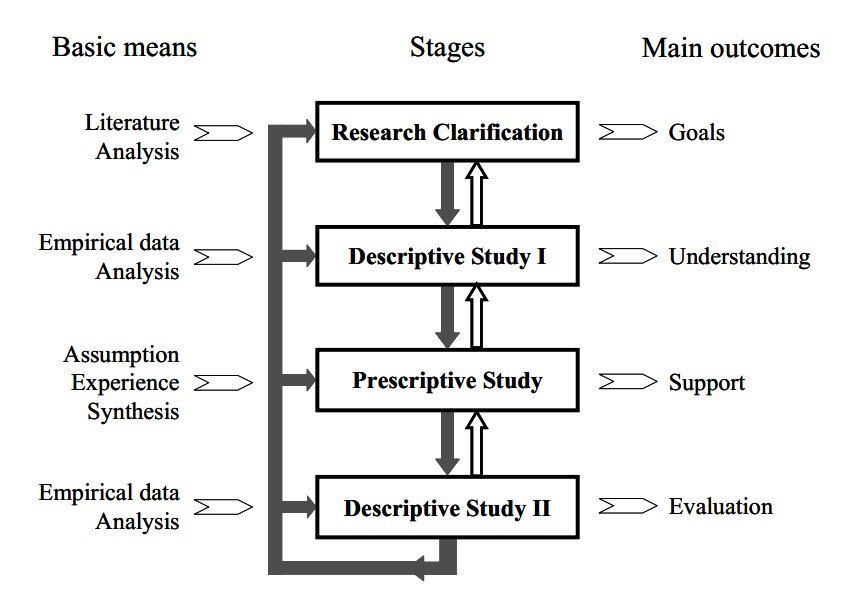
\includegraphics[scale=0.5]{DRMFramework.jpg}
        \caption{DRM Framework\cite{DRM.Framework}}
        \label{fig:DRM.Framework}
\end{figure}\par

DRM consists of four phases: Research Clarification, Descriptive Study I(DS I), Prescriptive Study (PS) and Descriptive Study II as mentioned in  Fig. \ref{fig:DRM.Framework} shows the links between these phases, the basic means used in each phase and the main outcomes. The bold arrows between the phases illustrate the main process flow, the light arrows the many iterations.
\begin{enumerate}
\item[1.]Research Clarification\par
%%In this phase author will be doing Literature Review study, to make problem identification and motive. In this phase author try to answer what does the main goal of this research topcis? Who needs this research? Why this research important?
In this phase, this study is trying to find some evidence or at least indications that support the assumptions in order to formulate a realistic and worthwhile research goal. the study does so mainly by searching the literature for factors that influence problem clarification. Based on the findings, an initial description of the existing situation is developed, as well as a description of the desired situation, in order to make the assumptions underlying each of the descriptions explicit. Initial reference model, initial impact model, preliminary criteria and overall research plan can be included in this phase.
\item[2.]Descriptive Study I\par
%%After having a clear goal and focus, author will review the literature for more influencing factor to elaborate the initial description of existing situation.
The intention of this phase is to make the description detailed enough to determine which factor(s) should be addressed to improve problem clarification as effectively and efficiently as possible. The analysis of the empirical data reveals the typical characteristics of insufficient problem definition and shows that insufficient problem definition in the problem-clarification phase is related to a high percentage of time spent on modifications in next phase of the process. This part may include by reference model and success criteria.
\item[3.]Prescriptive Study\par
%%In this stage, researcher will increased understanding of existing situation to correct and elaborate initial description and raised it into desired Situation
in this phase, this study uses the increased understanding of the existing situation to correct and elaborate o initial description of the desired situation. This description represents the vision on how addressing one or more factors in the existing situation would lead to the realisation of the desired, improved situation. This can develop various possible scenarios by varying the targeted factor(s). the study decides to focus on improving the quality of the problem definition as the most promising factor to address. this phase will be included impact model, support evaluation and outline evaluation plan. 
\item[4.]Descriptive Study II\par
the last phase is to investigate the impact of the support and its ability to realise the desired situation. Most of important point in this phase is evaluation. So, evaluation plan, application evaluation, success evaluation and implications are included in this phase. 
\end{enumerate}\par

\section{Research Workflow}
From the explanation of \ref{sec:ResearchDesign}, this research stand by the workflow below (Fig. \ref{fig:LangkahPenelitian}): \begin{enumerate}
\item[1.] Problems Identification. this stage becomes the important thing to be solved in this research. In this stage, the lack of synchronization between DM-related and non DM-regulation will be one of main problem to solved (mentioned at section \ref{sec:ResearchDesign}).
\item[2.] Literature Review. In this stage, the researcher collects many references from journals, articles, books or any informations related to problems stated at stage before.
\item[3.] Analysis and Identifications Solutions. There are many possible technologies can be used to solve the problem. In this phase, the researcher is trying to analyze and identify the best solution to used. 
\item[4.] Designing Model. Carried out in accordance with the results of analysis of technology solutions. Followed by architectural design, database, and display systems.
\item[5.] Prototyping. This stage is the stage of making a prototype of the analysis and design that has been generated from the previous process. Implementation is done in accordance with the tools and programming language that has been set. Implementation will be done only simulated and not all features will be implemented.
\item[6.] Testing. Performed to validate the system design. Tests conducted triangulation, namely through the black-box testing, simulation testing, and acceptance testing.
\item[7.] Evaluation. This stage is to look at the whole process of research and testing results to determine the conclusions of this study. Various suggestions may emerge from this evaluation stage.
\end{enumerate}\par
\begin{figure}[H]
\centering
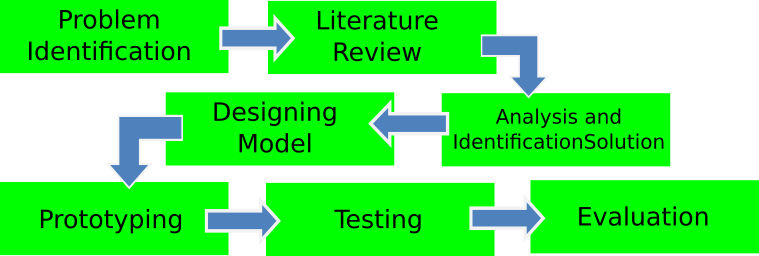
\includegraphics[scale=0.6]{LangkahPenelitian.png}
\label{fig:LangkahPenelitian}
\caption{Research Workflow}
\end{figure}\par
